\documentclass[mathserif]{beamer}

\usepackage{multicol}
\usepackage{beamerthemeshadow}
\usepackage{graphicx}
\usepackage{graphics}
\usepackage{pgf}
\usepackage{tikz}
\usepackage{hyperref}   % Hyperlink references and URLs
\usetikzlibrary{arrows,automata,petri,positioning}
\usepackage[latin1]{inputenc}

\title[AHOY: Slide \insertframenumber/\inserttotalframenumber]{AHOY: An event-based simulation environment}

\subtitle{Initial Presentation}

\author[Clark, Ingram, Kolakowska, \& Rosenfeld]{ 
Frank~Clark\inst{1}, Dustin~Ingram\inst{1}, Maria~Kolakowska\inst{1}, Aaron~Rosenfeld\inst{1}, William~Regli\inst{1}, Joseph~Macker\inst{2}, Michal~P\v{e}chou\v{e}k\inst{3}}

\institute{
    \inst{1}%
    Drexel University Department of Computer Science, Philadelphia PA
    \and
    \inst{2}%
    US Naval Research Laboratory Networks \& Communication Systems Branch, Washington DC
    \and
    \inst{3}%
    Czech Technical University Agent Technology Center, Prague
}

\date{\today}

\begin{document}

\frame{\titlepage} 

\frame
{
    \frametitle{Outline}
    \tableofcontents
}

\section{Motivation}

\subsection{Network Simulators}
\frame
{
    \frametitle{Background on Network Simulators}
    \begin{itemize}
        \item Application and protocol testing without physical hardware
        \item Mimic the properties of a physical network
        \item Network compents are virtualized (``nodes'') 
        \item Allow multiple virtual nodes to run on one physical machine
        \item Scale well, easy to re-configure
        \item Cost \& time effective
    \end{itemize}
}

\subsection{Agent Frameworks}
\frame
{
    \frametitle{Background on Agents \& Agent Frameworks}
    \begin{block}{Definition}
    An \emph{intelligent agent} is software which observes and acts upon an environment and directs its activity towards achieving goals (Russell, Norvig).
    \end{block}

    \textbf{Agent Simulators}
    \begin{itemize}
        \item Used to test agent algorithms within virtual worlds
        \item Rules define actions to be taken based on beliefs
        \item Agent rule-sets react to sensory information in the world
        \item Allows for large-scale simulation unfeasible in the real-world
    \end{itemize}
}

\subsection{Issues with Existing Tools}
\frame
{
    \frametitle{Existing tools}
    \textbf{Current Network Simulators}
    \begin{itemize}
        \item Designed for testing networks \& protocols, not agents 
        \item Scenarios are pre-scripted
        \item Poor event support
        \item Inability to vary settings across batch scenario executions
        \item Data collection non-existent or not directly supported
    \end{itemize}
    \textbf{Current Agent Frameworks}
    \begin{itemize}
        \item Communications modeled only at the application layer
        \item Lack of rich lower-level protocols, or
        \item Require physical hardware for networking
    \end{itemize}
}

\section{Implementation}

\subsection{Goals}
\frame
{
    \frametitle{Implementation Goals}
    \textbf{Bridge network simulators and agent simulators}
    \begin{itemize}
        \item Entirely event-driven
        \item Real-time
        \item Allow for human-in-the-loop interaction with agents
        \item Enable scenarios and network topologies to be easily defined
        \item Make writing custom agents extremely simple
        \item Visualization flexibility
        \item Physically distributed simulation
        \item Simple data collection
    \end{itemize}
}


\subsection{Overview}
\frame
{
    \frametitle{Overview of AHOY}
    \begin{itemize}
        \item AHOY is the realization of most of these goals
        \item Currently finished 2nd prototype iteration
        \item Key features:
        \begin{itemize}
            \item Event-Based Simulation
            \item Decoupled Visualization
            \item Scenario Setup \& Creation
            \item Scaled Distribution
            \item Batch Experimentation \& Data Collection
        \end{itemize}
    \end{itemize}
}

\frame
{
    \frametitle{Architecture}
    \begin{center}
        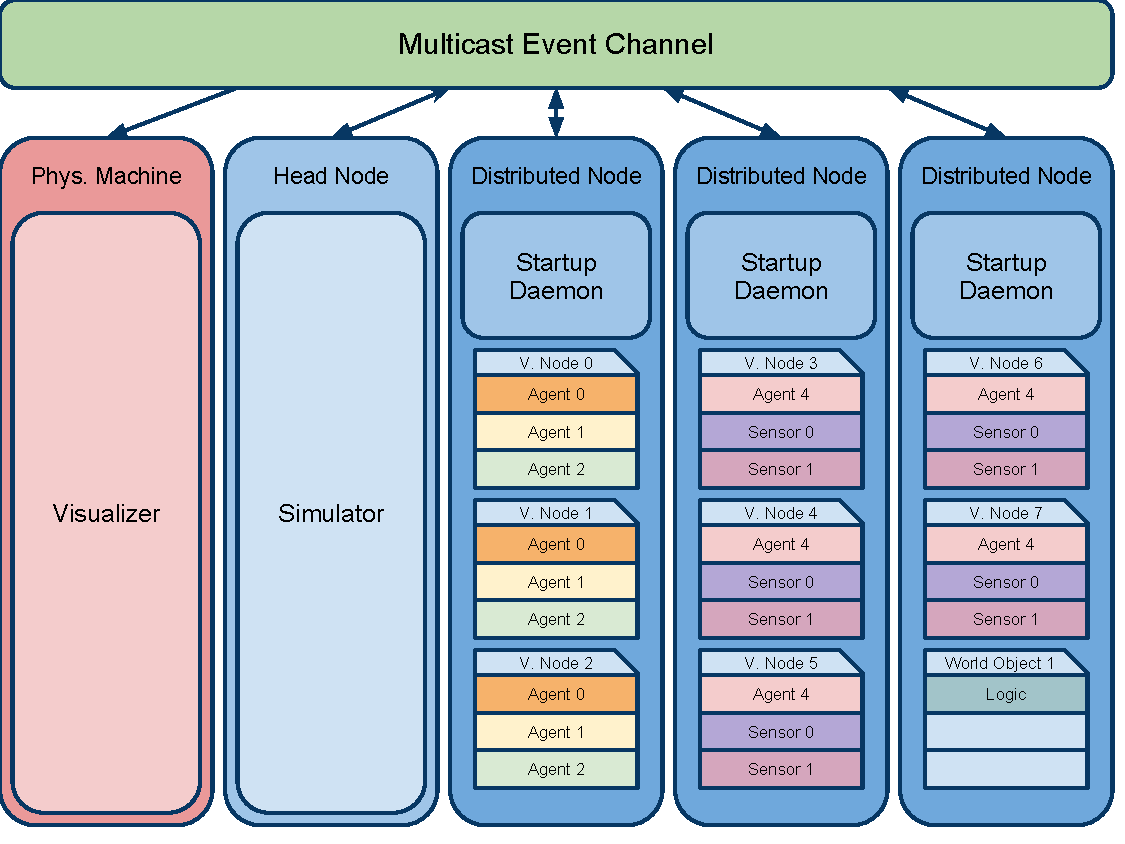
\includegraphics[scale=.48]{arch.pdf}
    \end{center}
}

\frame
{
    \frametitle{Event-Based Simulation}
    \textbf{Events allow Agents to react in real-time}
    \begin{itemize}
        \item Every action or change in the simulation is an event
        \item All events are passed over the event channel
        \item Event channel is available to all virtual nodes, agents
        \item Physical nodes as well, including visualizers
        \item New events can be inserted in real-time (human-in-the-loop)
    \end{itemize}
}

\frame
{
    \frametitle{Scaled Distribution}
    \textbf{Distribution of Virtual Nodes}
    \begin{itemize}
        \item Simple to distribute: everything is an event
        \item All events are broadcast over a common event channel
        \item Agents are started on multiple physical machines
    \end{itemize}
}

\frame
{
    \frametitle{Decoupled Visualization}
    \textbf{Visualizing the Simulation}
    \begin{itemize}
        \item Monitoring the event channel produces raw event data
        \item Occurs simultaneously with the execution of an experiment
        \item Visualizers interpret events, produce their own representation 
        \item Completely separated from the simulator
    \end{itemize}
}

\frame
{
    \frametitle{Scenario Setup \& Creation}
    \textbf{Using a ``Programming'' Interface}
    \begin{itemize}
        \item Each of the following are defined purely in Python:
        \begin{itemize}
            \item Agent Behaviors 
            \item Network Topologies
            \item Sensor Functionality
            \item World Objects \& Behaviors
        \end{itemize}
        \item These definitions are then interpreted by the simulator
        \item Sets up the experiment \& defines the scenario
    \end{itemize}

}

\frame
{
    \frametitle{Batch Experimentation}
    \textbf{Running Multiple Experiments \& Collecting Data}
    \begin{itemize}
        \item Users specify desired output metrics (e.g. lost packets)
        \item AHOY collects data during experiments and tabulates results
        \item Agent-specific metrics (e.g. algorithm performance) may be collected via the agent API
    \end{itemize}
}

\section{Demonstration}
\subsection{Prototype Demonstration}
\frame
{
    \frametitle{Prototype Demonstration}
    \textbf{A simple, multi-faceted scenario}
    \begin{itemize}
        \item 4 UAVs each controlled by a surveillance agent, 4 pre-scripted boats, 1 RADAR groundstation
        \item Wireless interfaces on each UAV; using log-loss model for pathloss
        \item RADAR takes into account cross-sectional area, Doppler shift, and shadowing
        \item Shows two visualizers working independently
        \item Human in the loop can change agents' behaviors
        \item Simulation distributed between two physical TUX nodes, each visualizer on an additional physical node
    \end{itemize}
}

\subsection{Q\&A}
\frame
{
    \frametitle{Q\&A}
    \begin{center} 
        \Huge Questions? 
    \end{center}
}

\frame
{
    \frametitle{Extra - Demo Architecture}
    \begin{center}
        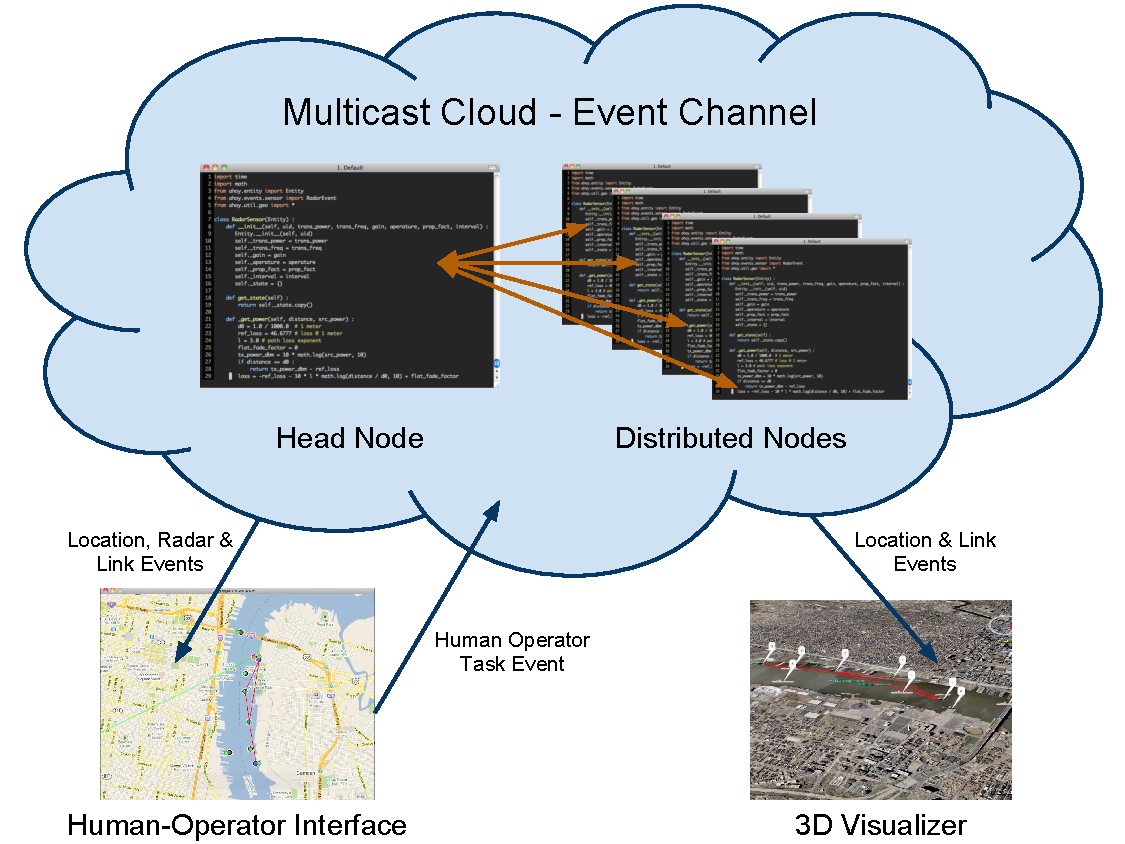
\includegraphics[scale=.48]{demo.pdf}
    \end{center}
}

\frame
{
    \frametitle{Extra - Demonstration Scenario}
    \begin{verbatim}
world = World()

wlan = Network('wlan0')
world.add_network(wlan)

heli_areas = [ ... ]
paths = [ ... ]

for i, loc in enumerate(heli_areas) :
    heli = Node(i)
    heli.set_position(loc[0], loc[1], feet(i * 100))
    heli.add_agent(RectangleSurveilAgent(heli, loc[0:2], loc[2:3], feet(150)))

    heli.add_interface(Interface('wlan0', heli, wlan, 120))
    world.add_entity(heli)

radar = RadarSensor2(len(world.get_entities()), watts(6000), 25, 1, 5, 1, 3/360.0, 1)
radar.set_position(39.9485, -75.1325, 0)
world.add_entity(radar)

for path in paths :
    e = Scripted(len(world.get_entities()), path[2:], path[0], 0)
    e.set_position(*path[1])
    world.add_entity(e)
    \end{verbatim}
}

\end{document}
